\chapter{Introduzione}

Elixir è un linguaggio di programmazione dinamico e funzionale
sviluppato nel 2012 da José Valim,
con l'obbiettivo di favorire uno sviluppo più agevole
sulla Erlang Virtual Machine(VM) e affrontare la sfida legata
a sistemi distribuiti, scalabili e affidabili mantenendo al
contempo la compatibilità con l'ecosistema di Erlang.
Elixir si è affermato come una promettente scelta
nell'industria del software,specialmente in contesti dove è
richiesta scalabilità, tolleranza agli errori e reattività 
grazie al suo approccio concorrenziale.

In particolare, Elixir può risultare vantaggioso nel
campo dell'IoT per diversi motivi:
\begin{enumerate}
	\item \textbf{Concorrenza}: Nell'ambito dell'IoT, la gestione
	simultanea di dispositivi è essenziale.
	Elixir, grazie alla concorrenza basata su processi leggeri,
	e tramite il modello basato su attori può consentire il monitoraggio
	e il controllo efficiente di numerosi dispositivi contemporaneamente.
	\item \textbf{Fault Tolerance}: 
	Data la natura degli ambienti IoT, dove i dispositivi possono
	guastarsi improvvisamente, Elixir offre strumenti per la supervisione
	e la gestione degli errori, garantendo la continuità delle operazioni
	anche in caso di fallimenti.
	\item \textbf{Sviluppo Rapido e Manutenzione}:
	Elixir è un linguaggio moderno che offre una sintassi efficiente e snella,
	oltre a strumenti di sviluppo come Mix per la gestione delle dipendenze
	e l'ambiente interattivo iex. La presenza di un package manager (Hex)\cite{Hex15:online}
	e la possibilità di generare automaticamente la documentazione
	facilitano il processo di sviluppo e manutenzione del codice.
	
\end{enumerate}

\section{IoT - L'internet delle cose}

L'Internet of Things (IoT),
traducibile in italiano come Internet delle cose,
si riferisce a un sistema di dispositivi interconnessi
attraverso una rete, capaci di raccogliere e scambiare
dati con sistemi esterni e di interagire con l'ambiente circostante.

Questi dispositivi possono essere 
dei sensori, telecamere, veicoli, elettrodomestici,
o qualsiasi altro oggetto in grado di comunicare
attraverso una rete.
L'obiettivo principale dell'IoT è quello di automatizzare processi,
migliorare l'efficienza, fornire informazioni in tempo reale
e creare nuove opportunità di servizi e applicazioni.

Un sistema IoT ha una vasta gamma di applicazioni ed il suo uso 
sta crescendo velocemente nella società moderna, basta pensare alle
molteplici applicazioni che spaziano dall'uso industriale
per l'automazione, all'uso individuale con la domotica.

\subsection{Architettura IoT}

Un'architettura base per l'IoT può essere composta da quattro
livelli come in figura \ref{fig:architettura_iot}

\begin{figure}[!htp]
    \centering
    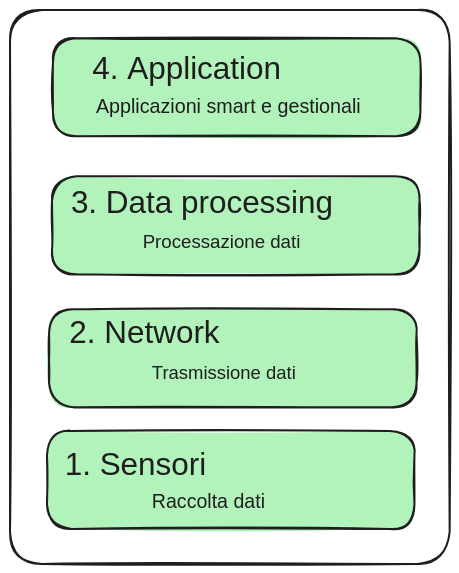
\includegraphics[keepaspectratio=true,scale=0.3]{images/architettura_iot.png}
	\caption{Architettura a 4 livelli}
  	\label{fig:architettura_iot}
\end{figure}

\begin{enumerate}
	\item Il livello Sensori è responsabile di collezionare dati da
	diverse sorgenti, i dispositivi fisici possono essere potenzialmente
	migliaia. Tutti questi dispositivi hanno il compito di
	inviare o ricevere dati ai livelli superiori.
	\item Il livello Network di un architettura IoT permette ai
	dispositivi di comunicare tra di loro o con il livello tre.
	Esempi di tecnologie di rete possono essere la rete WiFi,
	Zigbee e reti cellulari come il 5G.
	\item Il livello Data Processing gestisce la
	raccolta, l'analisi e l'interpretazione dei dati
	provenienti dai dispositivi IoT.
	Include tecnologie come sistemi di gestione dei dati,
	piattaforme di analisi e algoritmi di machine learning.
	\item Il livello delle applicazioni nell'architettura
	IoT è quello che interagisce direttamente con 
	l'utente finale, fornendo interfacce user-friendly 
	per controllare i dispositivi IoT. 
	Include app mobili, portali web e altre interfacce utente,
	oltre a servizi middleware per la comunicazione tra dispositivi.
	Inoltre, offre funzionalità di analisi e elaborazione dati,
	come algoritmi di machine learning e strumenti di visualizzazione.
\end{enumerate}

\subsubsection{Nerves}

Un framework open-source in Elixir
è Nerves \cite{NervesPr90:online}, consente di
sviluppare software embedded basato su Erlang/OTP.

Offre agli sviluppatori un ambiente di sviluppo 
coerente e potente per la creazione di firmware
e software per dispositivi IoT ed embedded.
Nerves semplifica il processo di sviluppo e distribuzione
di software per dispositivi embedded,
consentendo agli sviluppatori di creare
immagini firmware personalizzate e di integrare le funzionalità
richieste dai dispositivi.

Un esempio di utilizzo di Nerves nell'ambito IoT si ha
con l'azienda SparkMeter \cite{SparkMet65:online},
un azienda con l'obbiettivo di aumentare l'accesso all'elettricità
offrendo soluzioni di gestione della rete che 
consentono alle aziende di servizi pubblici nei mercati emergenti
di gestire sistemi finanziariamente sostenibili,
efficienti e affidabili.

I loro prodotti sono contatori elettrici
intelligenti e software di gestione della rete.
Questi possono essere utilizzati per misurare
il consumo di elettricità, raccogliere informazioni
sulla salute di una rete elettrica e gestire
la fatturazione.

Una panoramica della loro architettura è mostrata
in figura \ref{fig:architettura_spark}, dove sono
mostrati degli Smart Meters, dei sistemi embedded
responsabili di collezionare misure del consumo
dell'elettricità. Comunicano l'un l'altro tramite
una rete mesh e comunicano con il Grid Edge
management Unit, un altro sistema Embedded che
riceve e processa dati da migliaia di smart meters.
Il Grid Edge managmement unit comunica con il cloud
che processa i dati così da essere mostrati
da una User interface \cite{Embedded35:online}.
Sia il Grid Edge Management Unit che il server
fanno uso di Elixir, infatti l'infrastruttura
dei sistemi Embedded non sono affidabili, 
la rete per la comunicazione con cui comunicano i
dispositivi sono via radio,
possono diventare irraggiungibili per vari fattori,
come una mancanza di elettricità, guasto o mancanza di rete.
Il sistema così ha bisogno di essere Fault-tolerant ed è
uno dei cavalli di battaglia della piattaforma Erlang/OTP.
Inoltre utilizzando il meccanismo Port di Elixir,
vengono usati i vantaggi di Rust per processare
i dati dagli Smart Meters e processare i dati
in modo efficiente.

\begin{figure}[!htp]
    \centering
    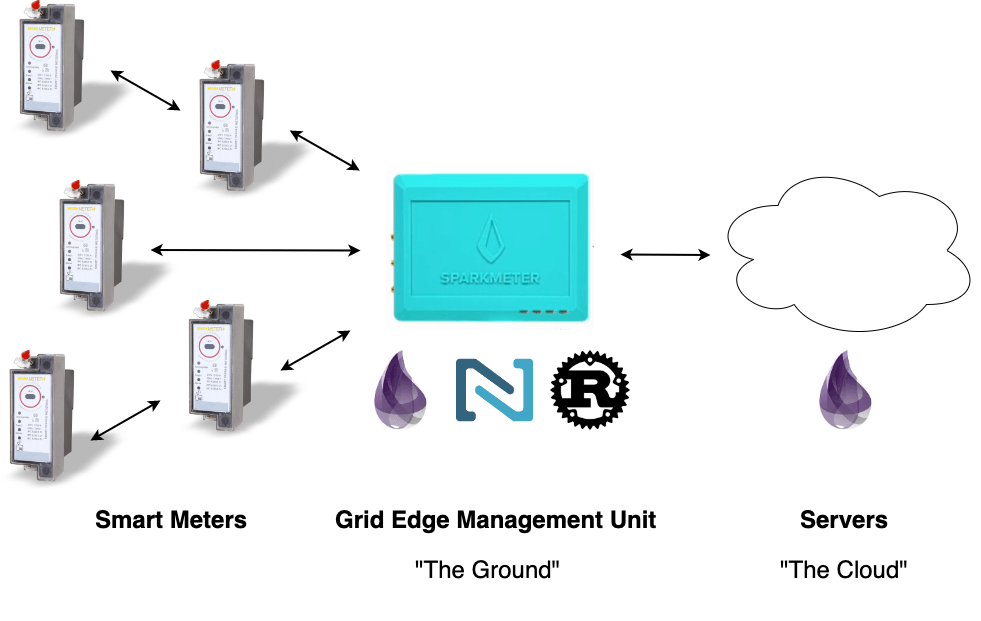
\includegraphics[keepaspectratio=true,scale=0.33]{images/sparkmeter-new-architecture.png}
	\caption{Un esempio di architettura IoT di SparkMeter\cite{Embedded35:online}}
  	\label{fig:architettura_spark}
\end{figure}



\subsection{Introduzione allo studio svolto}

Il trattato esplora Elixir concentrandosi su due aspetti principali:
la semplicità e le performance. Si analizzano i punti di forza di 
un linguaggio funzionale e come questi sono sfruttati in Elixir, con 
un focus sulla concorrenza. Nella scelta di un linguaggio, la semplicità
è fondamentale e deve essere accessibile a tutti i programmatori.
Tuttavia, l'efficienza è altrettanto importante, quindi vengono condotti
test empirici per valutare le performance di Elixir.

In particolare il lavoro effettuato è così ripartito: 


\begin{itemize}
	\item Nel capitolo 2 si discute del linguaggio funzionale,
	esaminando le astrazioni offerte da Elixir per lo svilluppo
	di codice fault tolerant, si tratta la concorrenza e come la Erlang VM
	si occupa della gestione dei processi.
	\item Nel capitolo 3 si spiega il lavoro sperimentale svolto e i risultati
	ottenuti, in particolare vengono effettuati quattro test, i primi due
	per valutare l'efficienza della concorrenza della VM, il terzo per
	sperimentare l'interoperabilità con il codice C/C++ confrontando le
	performance del codice C/C++ con quello di Elixir, infine,nel quarto test
	si misura il throughput di un server Http scritto in
	Elixir confrontandolo con dei semplici server scritti in Node e Python

\end{itemize}


